%%%%%%%%%%%%%%%%%%%%%%%%%%%%%%%%%%%%%%%%%%%%%%%%%%%%%%%%%%%%%%%%%%%%%%%%%%%%%%%%%%%%%%%%%%%%%%%%%
%
% Document:      DM  product tree
%
%%%%%%%%%%%%%%%%%%%%%%%%%%%%%%%%%%%%%%%%%%%%%%%%%%%%%%%%%%%%%%%%%%%%%%%%%%%%%%
\documentclass{article}
\usepackage{times,layouts}
\usepackage{tikz,hyperref,amsmath}
\usetikzlibrary{positioning,arrows,shapes,decorations.shapes,shapes.arrows}
\usetikzlibrary{backgrounds,calc}
\usepackage[paperwidth=31cm,paperheight=60cm,
left=-2mm,top=3mm,bottom=0mm,right=0mm,
noheadfoot,marginparwidth=0pt,includemp=false,
textwidth=30cm,textheight=50mm]{geometry}
\newcommand\showpage{%
\setlayoutscale{0.5}\setlabelfont{\tiny}\printheadingsfalse\printparametersfalse
\currentpage\pagedesign}
\hypersetup{pdftitle={DM organisation }, pdfsubject={Diagram illustrating the
products in LSST DM }, pdfauthor={ William O'Mullane}}
\tikzstyle{wbbox}=[rectangle, rounded corners=3pt, draw=black, top color=blue!50!white, bottom color=white, very thick, minimum height=12mm, inner sep=2pt, text centered, text width=30mm] 
\tikzstyle{pbox}=[rectangle, rounded corners=3pt, draw=black, top color=yellow!50!white, bottom color=white, very thick, minimum height=12mm, inner sep=2pt, text centered, text width=30mm] 
\tikzstyle{pline}=[-, thick]\begin{document}
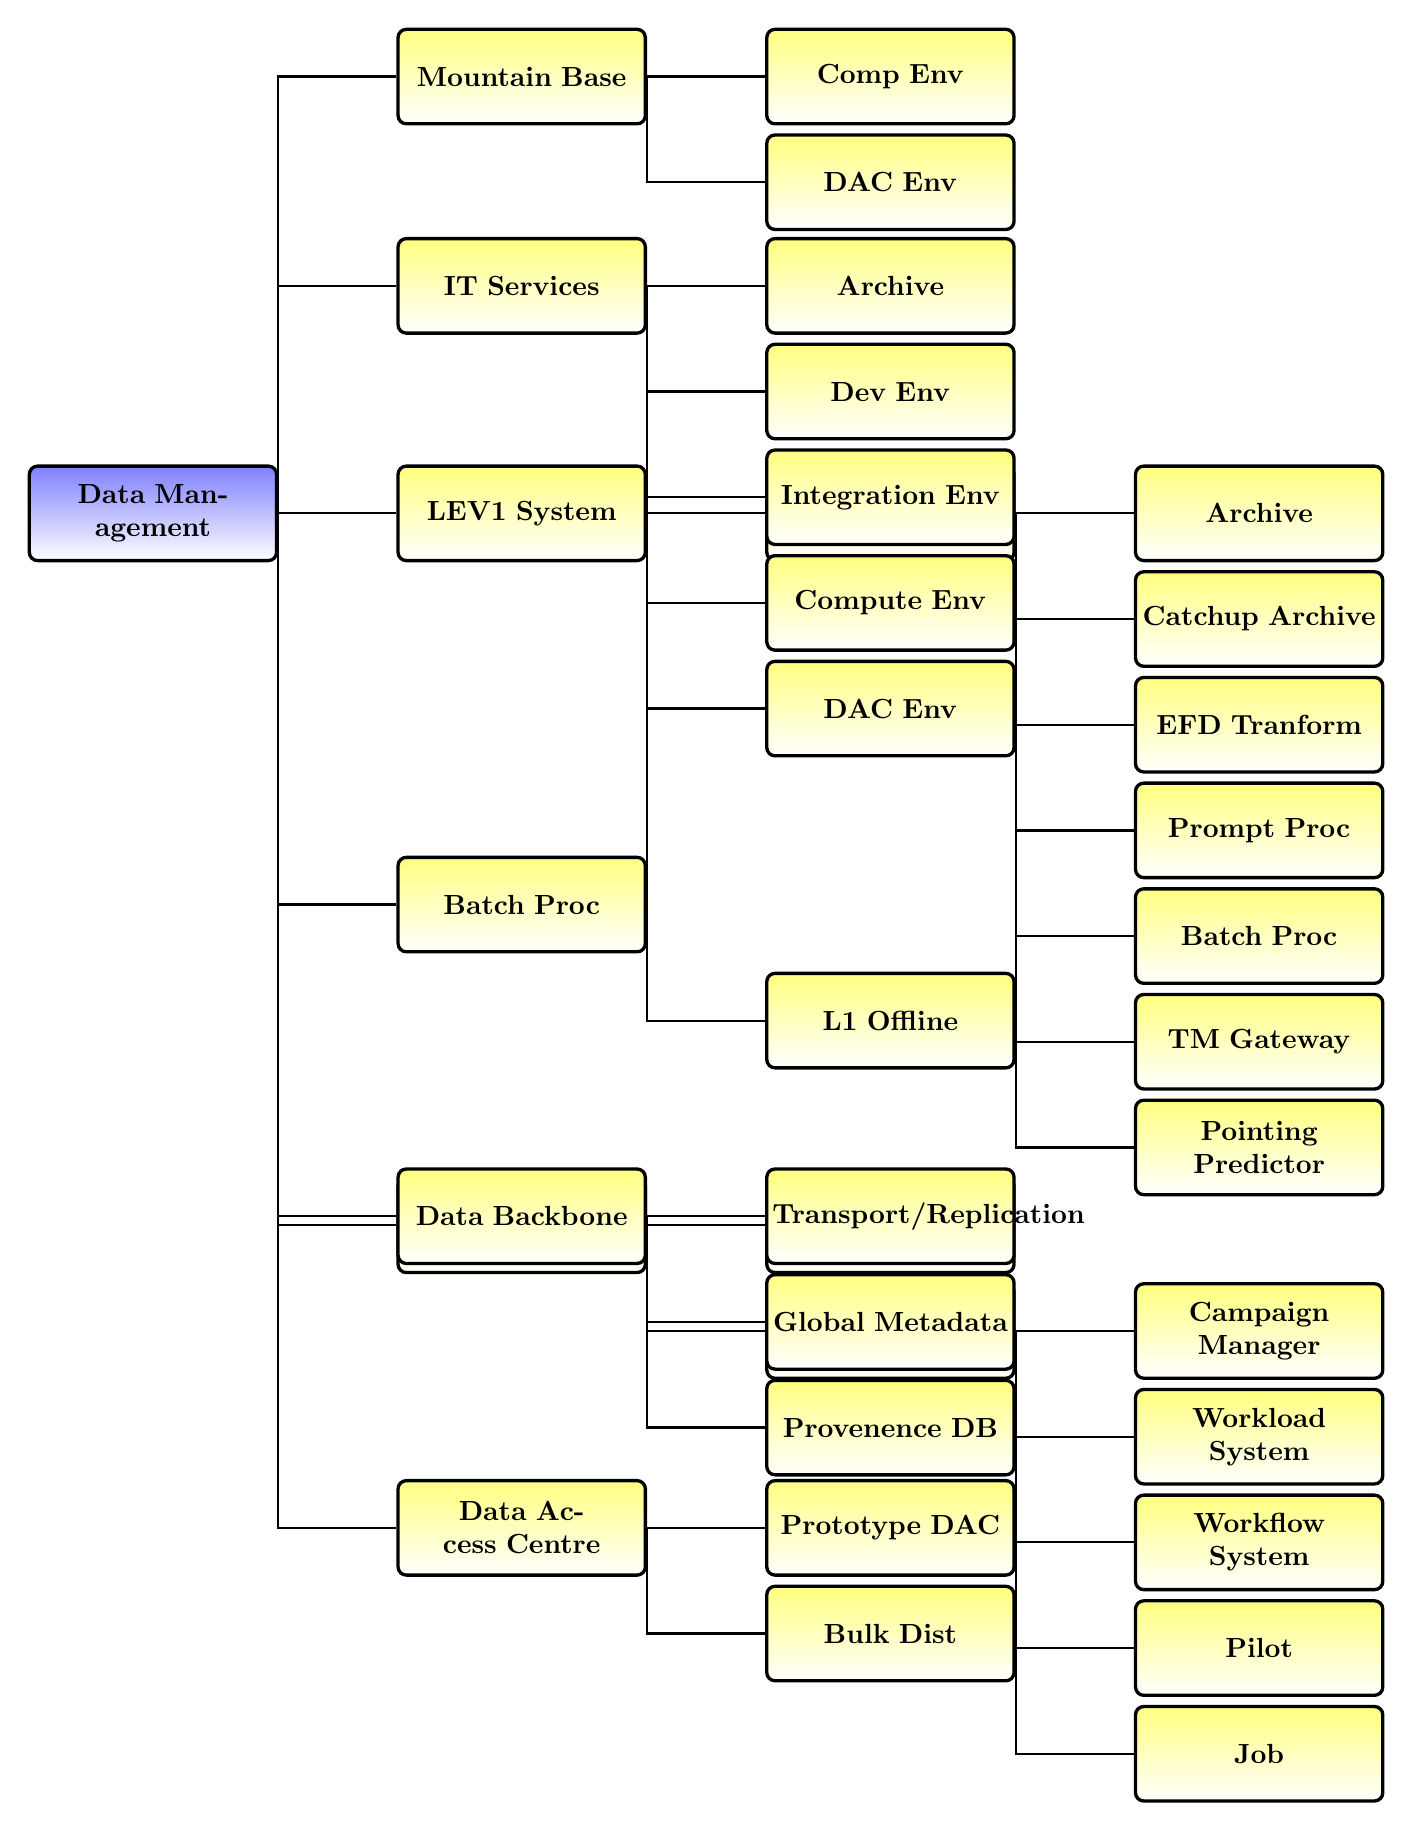
\begin{tikzpicture}[node distance=0mm]
\node (DM) [wbbox]{\textbf{Data Management}}; 
\node (L1) [pbox,right=15mm of DM] {\textbf{LEV1 System}}; 
 \draw[pline] (L1.west) -| (DM.east);
 \node (L1OCS) [pbox,right=15mm of L1] {\textbf{L1 OCS}}; 
 \draw[pline] (L1OCS.west) -| (L1.east);
 \node (ARC) [pbox,right=15mm of L1OCS] {\textbf{Archive}}; 
 \draw[pline] (ARC.west) -| (L1OCS.east);
 \node (CARC) [pbox,below=1mm of ARC] {\textbf{Catchup Archive}}; 
 \draw[pline] (CARC.west) -| (L1OCS.east);
 \node (EFDT) [pbox,below=1mm of CARC] {\textbf{EFD Tranform}}; 
 \draw[pline] (EFDT.west) -| (L1OCS.east);
 \node (PRMP) [pbox,below=1mm of EFDT] {\textbf{Prompt Proc}}; 
 \draw[pline] (PRMP.west) -| (L1OCS.east);
 \node (BP) [pbox,below=1mm of PRMP] {\textbf{Batch Proc}}; 
 \draw[pline] (BP.west) -| (L1OCS.east);
 \node (TMG) [pbox,below=1mm of BP] {\textbf{TM Gateway}}; 
 \draw[pline] (TMG.west) -| (L1OCS.east);
 \node (POINTP) [pbox,below=1mm of TMG] {\textbf{Pointing Predictor}}; 
 \draw[pline] (POINTP.west) -| (L1OCS.east);
 \node (L1OFF) [pbox,below=52mm of L1OCS] {\textbf{L1 Offline}}; 
 \draw[pline] (L1OFF.west) -| (L1.east);
 \node (L2) [pbox,below=78mm of L1] {\textbf{LEV2 System}}; 
 \draw[pline] (L2.west) -| (DM.east);
 \node (CAL) [pbox,right=15mm of L2] {\textbf{Calibration}}; 
 \draw[pline] (CAL.west) -| (L2.east);
 \node (DRP) [pbox,below=1mm of CAL] {\textbf{Data Release Prod}}; 
 \draw[pline] (DRP.west) -| (L2.east);
 \node (CM) [pbox,right=15mm of DRP] {\textbf{Campaign Manager}}; 
 \draw[pline] (CM.west) -| (DRP.east);
 \node (WLS) [pbox,below=1mm of CM] {\textbf{Workload System}}; 
 \draw[pline] (WLS.west) -| (DRP.east);
 \node (WFS) [pbox,below=1mm of WLS] {\textbf{Workflow System}}; 
 \draw[pline] (WFS.west) -| (DRP.east);
 \node (PILOT) [pbox,below=1mm of WFS] {\textbf{Pilot}}; 
 \draw[pline] (PILOT.west) -| (DRP.east);
 \node (JOB) [pbox,below=1mm of PILOT] {\textbf{Job}}; 
 \draw[pline] (JOB.west) -| (DRP.east);
 \node (DAC) [pbox,below=26mm of L2] {\textbf{Data Access Centre}}; 
 \draw[pline] (DAC.west) -| (DM.east);
 \node (PDAC) [pbox,right=15mm of DAC] {\textbf{Prototype DAC}}; 
 \draw[pline] (PDAC.west) -| (DAC.east);
 \node (BULKD) [pbox,below=1mm of PDAC] {\textbf{Bulk Dist}}; 
 \draw[pline] (BULKD.west) -| (DAC.east);
 \node (DBB) [pbox,below=-52mm of DAC] {\textbf{Data Backbone}}; 
 \draw[pline] (DBB.west) -| (DM.east);
 \node (DTR) [pbox,right=15mm of DBB] {\textbf{Transport/Replication}}; 
 \draw[pline] (DTR.west) -| (DBB.east);
 \node (GMDS) [pbox,below=1mm of DTR] {\textbf{Global Metadata}}; 
 \draw[pline] (GMDS.west) -| (DBB.east);
 \node (PRDB) [pbox,below=1mm of GMDS] {\textbf{Provenence DB}}; 
 \draw[pline] (PRDB.west) -| (DBB.east);
 \node (BPS) [pbox,below=-52mm of DBB] {\textbf{Batch Proc}}; 
 \draw[pline] (BPS.west) -| (DM.east);
 \node (ITS) [pbox,below=-91mm of BPS] {\textbf{IT Services}}; 
 \draw[pline] (ITS.west) -| (DM.east);
 \node (ITARC) [pbox,right=15mm of ITS] {\textbf{Archive}}; 
 \draw[pline] (ITARC.west) -| (ITS.east);
 \node (DENV) [pbox,below=1mm of ITARC] {\textbf{Dev Env}}; 
 \draw[pline] (DENV.west) -| (ITS.east);
 \node (INTENV) [pbox,below=1mm of DENV] {\textbf{Integration Env}}; 
 \draw[pline] (INTENV.west) -| (ITS.east);
 \node (COMPENV) [pbox,below=1mm of INTENV] {\textbf{Compute Env}}; 
 \draw[pline] (COMPENV.west) -| (ITS.east);
 \node (DACENV) [pbox,below=1mm of COMPENV] {\textbf{DAC Env}}; 
 \draw[pline] (DACENV.west) -| (ITS.east);
 \node (BASE) [pbox,below=-39mm of ITS] {\textbf{Mountain Base}}; 
 \draw[pline] (BASE.west) -| (DM.east);
 \node (BCOMPENV) [pbox,right=15mm of BASE] {\textbf{Comp Env}}; 
 \draw[pline] (BCOMPENV.west) -| (BASE.east);
 \node (BDACENV) [pbox,below=1mm of BCOMPENV] {\textbf{DAC Env}}; 
 \draw[pline] (BDACENV.west) -| (BASE.east);
   no parent 
\end{tikzpicture}
\end{document}
